% 论文正文是主体,主体部分应从另页右页开始,每一章应另起页。一般由序号标题、文字叙述、图、表格和公式等五个部分构成。
\section{绪论}
\subsection{研究背景与意义}

``人类基因组计划"的研究引发后基因组时代的到来,标志着生命科学开始进入系统生物学时代,
人们开始研究各种组学在 DNA、mRNA、蛋白质和各种代谢产物水平上研究各种分子的生物功能。
系统生物学首先通过生物学技术对系统进行干涉,并利用物理、化学实验方法测量得到实验数据,
然后将这些数据用计算机存储起来,最后运用数学、物理方法结合计算机技术对这些数据进行统计、分析,
利用数学理论建立生物系统模型。
所以系统生物学研究的的方法和手段,决定了系统生物学是一个物理、化学、数学、信息学、计算机科学和分子生物学等多学科交叉学科,
需要各种学科的密切配合 \cite{ideker2001new}。

在系统生物学上,基础和核心问题之一是理解和认识能够代表基因发育和调控过程因果关系的基因调控网络 (Gene Regulatory Networks, GRNs)。
基因调控网络描述的是细胞或组织内复杂的生命过程中的功能通路,比如新陈代谢、基因调控、运输机制或者信号传导。
从宏观上看,基因调控网络是由细胞中参与基因调控作用的 DNA、RNA、蛋白质以及代谢中间物所形成的相互作用的网络 \cite{de2002modeling}。
从微观上看,一个基因的转录由细胞的生化状态所决定,在一个基因的转录过程中,一组转录因子作用于该基因的启动子区域,
控制该基因转录,而这些转录因子本身又是其它基因的产物。
当一个基因通过转录、翻译形成功能基因产物后,它将改变细胞的生化状态,
从而直接或间接地影响其它基因的表达或者自身的表达。
多个基因的表达不断变化,使得细胞的生化状态不断地变化,构成复杂的基因调控网络。
图 \ref{cover-2} 展示了从宏观上对应的生物过程 (Biological Reality) 到微观上对应的抽象模型 (Abstract Model) 的一个实例。
总体而言,基因调控具有如下三个特征: 
(1) 调控方式多样化: 既存在一对一的基因之间的调控,也存在一对多或多对一的多因子调控;
(2) 类型多样性,可由 DNA、RNA、蛋白质、小分子等多种类型参与;
(3) 调控关系动态变化。

\begin{figure}[!htbp]
    \centering
    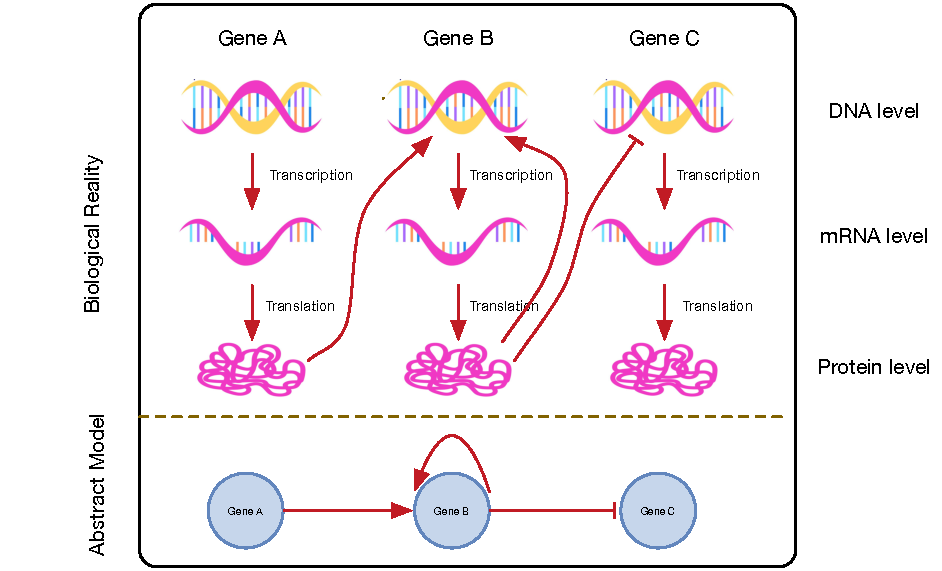
\includegraphics[width=0.95\textwidth]{cover-2.pdf}
    \caption{GRNs 构建的主要目标是为实际生物过程生成抽象模型。
    这些模型试图表示生物过程分子实体之间复杂的相互作用,比如基因激活、抑制或反馈环路。
    }
    \label{cover-2}
\end{figure}

在实际研究抽象模型的时候,从计算建模上,基因调控网络可以用不同类型的图来表示:
如果是无向图,该网络表示的是基因和基因之间的相互依赖结构。
如果是有向图,该网络除了表示结构之外还蕴含了基因之间的调控关系。
显然,构建有向图比构建无向图难度更高,挑战更大。
图 \ref{cover-1} 表示的是一个典型的有向的基因调控网络,节点表示基因, 边代表的是基因之间的调控关系。
需要说明的是,在本文的研究中不刻意区分调控中的激活 (activating) 或抑制 (inhibiting) 关系,
也就是说基因调控间的激活或者抑制都视为基因之间存在调控关系。
\begin{figure}[!htbp]
    \centering
    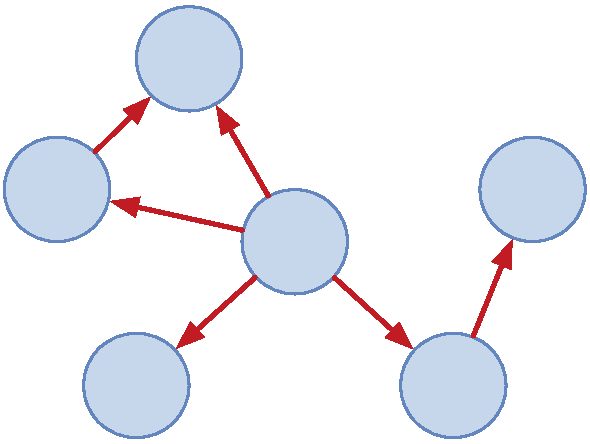
\includegraphics[width=0.5\textwidth]{cover-1.pdf}
    \caption{GRNs 示例图。节点表示基因, 边代表的是基因之间的调控关系。}
    \label{cover-1}
\end{figure}

从数据上,微阵列芯片 (microarray) 技术和单细胞 RNA测序 (scRNA-seq) 技术的发展产生的大量基因表达数据,
这些基因表达数据不仅可用于分析基因表达的时空规律,研究基因的功能,而且还可用于基因之间的相互制约关系,
研究基因调控网络模型,为理解生物潜在的调控机制带来了机遇。
另外, 转录组学、蛋白质组学、相互作用组学、代谢组学等高通量的实验室技术可以为模型提供更多的先验信息,
有助于构建更加复杂、更准确地反应生命现象的基因调控动态网络。

构建基因调控网络的直接目标是利用基因表达数据来学习和挖掘基因间的调控关系,并借助于可视化技术展现基因调控网络的拓扑结构。
基因调控网络的构建,有助于我们从网络的角度去了解复杂而精密的生物网络系统所蕴涵的结构和功能信息,
促进我们发现基因新的功能,预测和疾病相关的潜在的基因 \cite{lee2009computational},分析细胞代谢通路,
在分子水平上理解癌症发生的机理,
揭示癌症的内部机制,进一步增强我们对癌症的整体认识,
甚至是诊断、控制和治疗癌症的方法 \cite{kreeger2009cancer,yan2016biological}。
另外,从计算的角度看,基因调控网络的构建有助于我们节省大量的实验费用与资源,
也可以利用模拟结果有效地指导进一步的生物实验,
尤其是在肿瘤等复杂疾病研究 \cite{boyle2017expanded},
例如癌症细胞的分化、扩散和增生、肿瘤药物的筛选和研制等 \cite{hurley2011gene},为攻克癌症等复杂疾病做出贡献。

总之, 基因调控网络构建是一门理论研究与实践应用相结合的学科,它不仅有重要的学术意义,
还有很高的商业价值,以及广阔的发展前景。
随着后基因组时代的到来,基因调控网络不仅可以为生物信息学提供大量的研究线索,
也可为特定生物问题提供强有力的理论依据,还可在疾病诊断、药物筛选等领域发挥更加广泛的作用 \cite{kreeger2009cancer}。

\subsection{国内外研究现状和发展动态}

基因调控网络构建是一种依靠数据挖掘进行的逆向工程研究, 即根据基因表达数据推理基因调控网络中的各类拓扑结构。
它首先通过生物实验获取高通量生物数据, 然后根据生物网络的先验知识, 针对特定生物问题建立数学模型, 
并设计合理的算法构建基因调控网络, 最后通过生物学实验验证逐步逼近和发现真实的基因调控网络 \cite{sima2009inference}。
从计算角度讲,基因调控网络构建依赖于已知的知识数据库发现 (Knowledge Database Discovery, KDD) 工作流程。
KDD 从输入数据预处理到模型的验证,通过数据库搜索比较之前的实验数据结果来完成的,总计包含六个步骤,如图 \ref{cover-3} 所示。
\begin{figure}[!htbp]
    \centering
    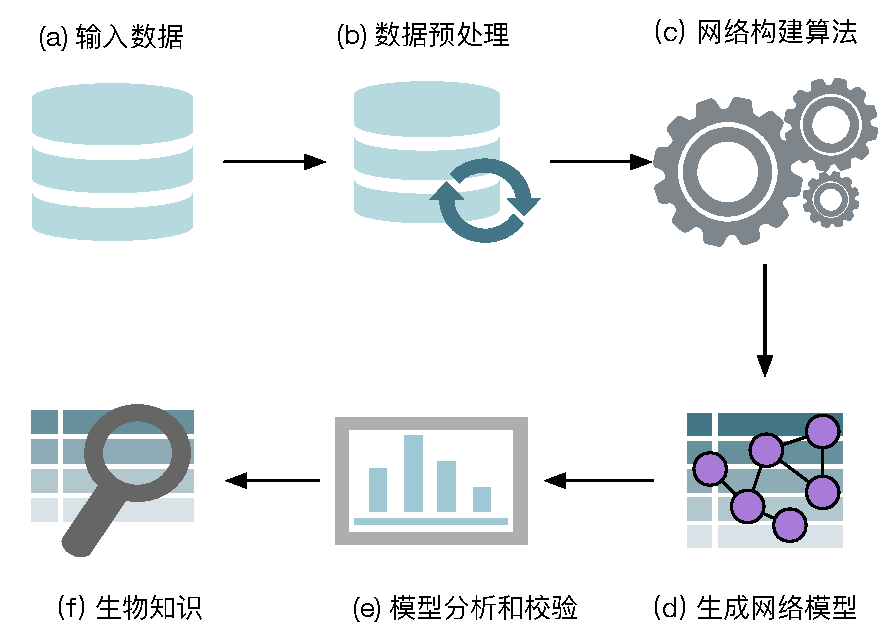
\includegraphics[width=0.8\textwidth]{kdd-cn.pdf}
    \caption{基于 KDD 工作流程的 GRN 重建步骤。}
    \label{cover-3}
\end{figure}

当前的基因调控网络构建牵涉到三方面的研究问题 \cite{schlitt2007current}:
(1) 根据数据源建立什么样的网络模型?
(2) 如何设计与实现网络构建算法?
(3) 如何评价和甚至是应用构建的网络?
第三个方面属于应用范畴的研究,不是本文研究的重点, 因此我们仅从前两个方面讨论基因调控网络构建的相关研究现状。
同时由于大多数方法是跟数据特性密切相关, 因此本文将首先介绍下数据源及其特征。

\subsubsection{数据源}

网络模型的建立首先需要我们对现在测序技术产生的数据及其特征有充分的认识。
在过去十几年中,高通量技术提供了巨大的数据,诸如下一代测序技术 (Next Generation Sequencing, NGS) \cite{BUERMANS20141932}, 
产生了显著质量、稳健性和低噪声的 DNA 和 RNA 样本数据。
测序已经成为一种标准方法,被认为是研究生命体的基石 \cite{CEREB2015923}。
测序产生的基因表达数据使生物学家能够大规模观察基因的表达水平, 对构建基因调控网络起到了至关重要的作用。
基因表达数据来源包括 DNA 微阵列, RNA-seq \cite{morin2008profiling}和 SAGE (基因表达系列分析) \cite{velculescu1995serial}。
在基因调控网络构建中我们将主要使用 DNA 微阵列数据 (microarray data) 和单细胞 RNA-seq 数据 (scRNA-seq),
同时也会结合其它比如 PPI (蛋白质相互作用网络) 数据, TF (转录因子) 结合位点数据等作为先验知识。

(1) DNA 微阵列测序数据

DNA 微阵列技术(DNA microarray) 是上个世纪 90 年代产生的最为重要的基因测序技术,
是分子生物学在实验领域的重大突破,为探索生命本质和奥秘提供了基础保障。
该技术是在固相支持物表面集成大量的分子探针,与标记好的样品杂交,
来测定细胞内 mRNA 内的表达量也就是基因表达谱 (Gene Expression Profiles),
在不同条件下不同发展阶段和不同组织中的转录水平。
该技术能在同一时间内高效快速地分析大量基因的表达水平。
基因表达谱中蕴含了非常珍贵的信息,可以分析哪些基因的表达发生了更改, 
基因之间的表达有无相关性,基因的变化会对细胞产生怎样的变化,进而能帮助人们深入地认识诸如基因表达调控、发育、
疾病与癌症病理、衰老等生物过程 \cite{chen2005selecting,shen2009new,camargo2008identification}。
基因表达谱数据天生就具有小样本、高维度、高噪声高变异和非线性四个分析和处理上的难点。
高维度和小样本,使得基因表达数据处理时存在``维度诅咒"的问题 \cite{wang2006inferring}。
高噪声高变异和非线性等使得数据信息的挖掘提取更具有难度。
所有的这些问题使得准确构建基因之间的调控相互作用,
尤其是在后基因组时代处理大规模基因表达数据时,
变得更加复杂和具有挑战性。

(2) 单细胞 RNA-seq 数据

单细胞 RNA-seq 技术在 2009年首先由 Tang等 \cite{tang2009mrna}提出,
但是在 2014 年以后由于新的协议和相对低廉的测序成本使得它在产业界和学术界都颇受欢迎,风靡至今。
单细胞 RNA-seq 技术与 DNA 微阵列测序技术最为显著的不同是,
后者测量的基因表达值是多个细胞基因表达值的平均值,
而前者测量的是单个细胞中的基因表达值。
单细胞 RNA-seq 测序技术也给数据处理带来诸多挑战,
比如大量的细胞异质性 \cite{wagner2016revealing},高度稀疏性导致的表达为零 (dropout\footnote{单细胞领域的 dropout 跟深度学习里面的 dropout 不是一个含义}) \cite{vallejos2017normalizing}, 细胞与细胞之间的测序深度变化, 细胞周期相关的批量效应 (batch effects) \cite{buettner2015computational}。
在数据预处理阶段, 需要实现的目标不同和数据产生的场景, 对基因的 dropout值进行过滤或者填充 (dropout imputation), 或者需要对数据进行批量校正 (batch effects correction), 以提高后续下游分析的稳定性。
单细胞 RNA-seq 技术可以用来研究在转录组细胞特异性的变化中重要和新的生物学问题,
如鉴定细胞类型, 研究基因表达的随机性, 细胞发育轨迹推断 (trajectory inference),与细胞类型或者周期相关的基因调控网络的推断。
相比于微阵列测序数据而言,大多数情况下单细胞 RNA-seq 数据的计算分析需要开发新的方法。

\subsubsection{网络模型}

寻找一个合适的网络模型是构建网络的首要问题。
在基因调控网络的研究中,为刻画和反应复杂生物网络的动态或静态行为,数学模型提供了一个强有力的工具。
不同的数学模型对基因调控网络进行了不同的表达和抽象,然而针对复杂的基因调控网络,
为对其进行全面描述,需要借助多个层次多种类型的模型来反应基因调控网络的不同特性。

从时空特性上区分,基因调控网络模型可分为:
静态模型与动态模型,例如,动态贝叶斯网是动态模型;
从图论角度区分,分为有向图模型和无向图模型;
从网络拓扑特性的角度出发,可构造出复杂网络和差异网络的模型。 
从建模所用的数据区分,模型可分为:
离散模型与连续模型,时序模型与非时序模型。
上面介绍的在基因调控网络构建中使用的两大类数据, DNA 微阵列测序数据和单细胞 RNA-seq 数据, 
可以划分为时间序列数据 (time series data) 和非时序的扰动实验数据 (perturbation experiments data) 两种。
时间序列表达数据使生物学家能够调查生物网络中的时间模式,适合用来构建时序模型, 比如可采用微分方程模型建模; 
扰动表达数据提供了关于基因间调控方向的信息。
在单细胞数据中,序列的时间也可以是伪时间的, 比如在细胞发育轨迹推断中经常需要依赖伪时间推断算法, 来对细胞的时间先后及间隔进行标注。
非时序的扰动实验分为两类:基因操作 (即基因缺失,过度表达,温度敏感或动力学突变) \cite{holstege1998dissecting} 或外部处理 (即环境胁迫) \cite{gasch2000genomic}。

随着数据来源的多样化,模型改进和模型组合是当前网络模型的主要研究方向。
模型改进是针对现有的模型引入新的法则来构造新的模型,
而模型组合则是结合几个不同类型的模型取长补短达到性能最优。

\subsubsection{网络构建算法}
研究者们提出的基因调控网络的各类模型都在不同层次、不同程度上对真实的调控网络进行了抽象,
目前已提出的主要基因调控网络构建方法有关联网络、布尔网络、微分方程、贝叶斯网络、动态贝叶斯网络、回归方法。
接下来,本文将对这些方法的优缺点以及对应的研究现状做简要介绍。

(1) 布尔网络

布尔网络与微分方程相比则更为抽象,它对基因的状态做了进一步的简化,
用布尔函数代替了微分和导数来描述基因间的相互作用关系 \cite{shmulevich2002probabilistic,kim2007boolean,bornholdt2008boolean,zhou2016relative} 。
其中,基因的状态定量为两种不同的状态(``开"和``关")。
状态``开"表示一个基因转录表达, 状态``关"则代表一个基因未转录。
如果布尔网络模型进一步推广, 其可转变为时序布尔网络模型 TBN (temporal Boolean networks), 这有利于处理多于一个单位时间跨度的基因间的依赖性。
图 \ref{fig:pre-bn} 展示了使用布尔模型方法的整体的工作流程。
\begin{figure}[!htbp]
    \centering
    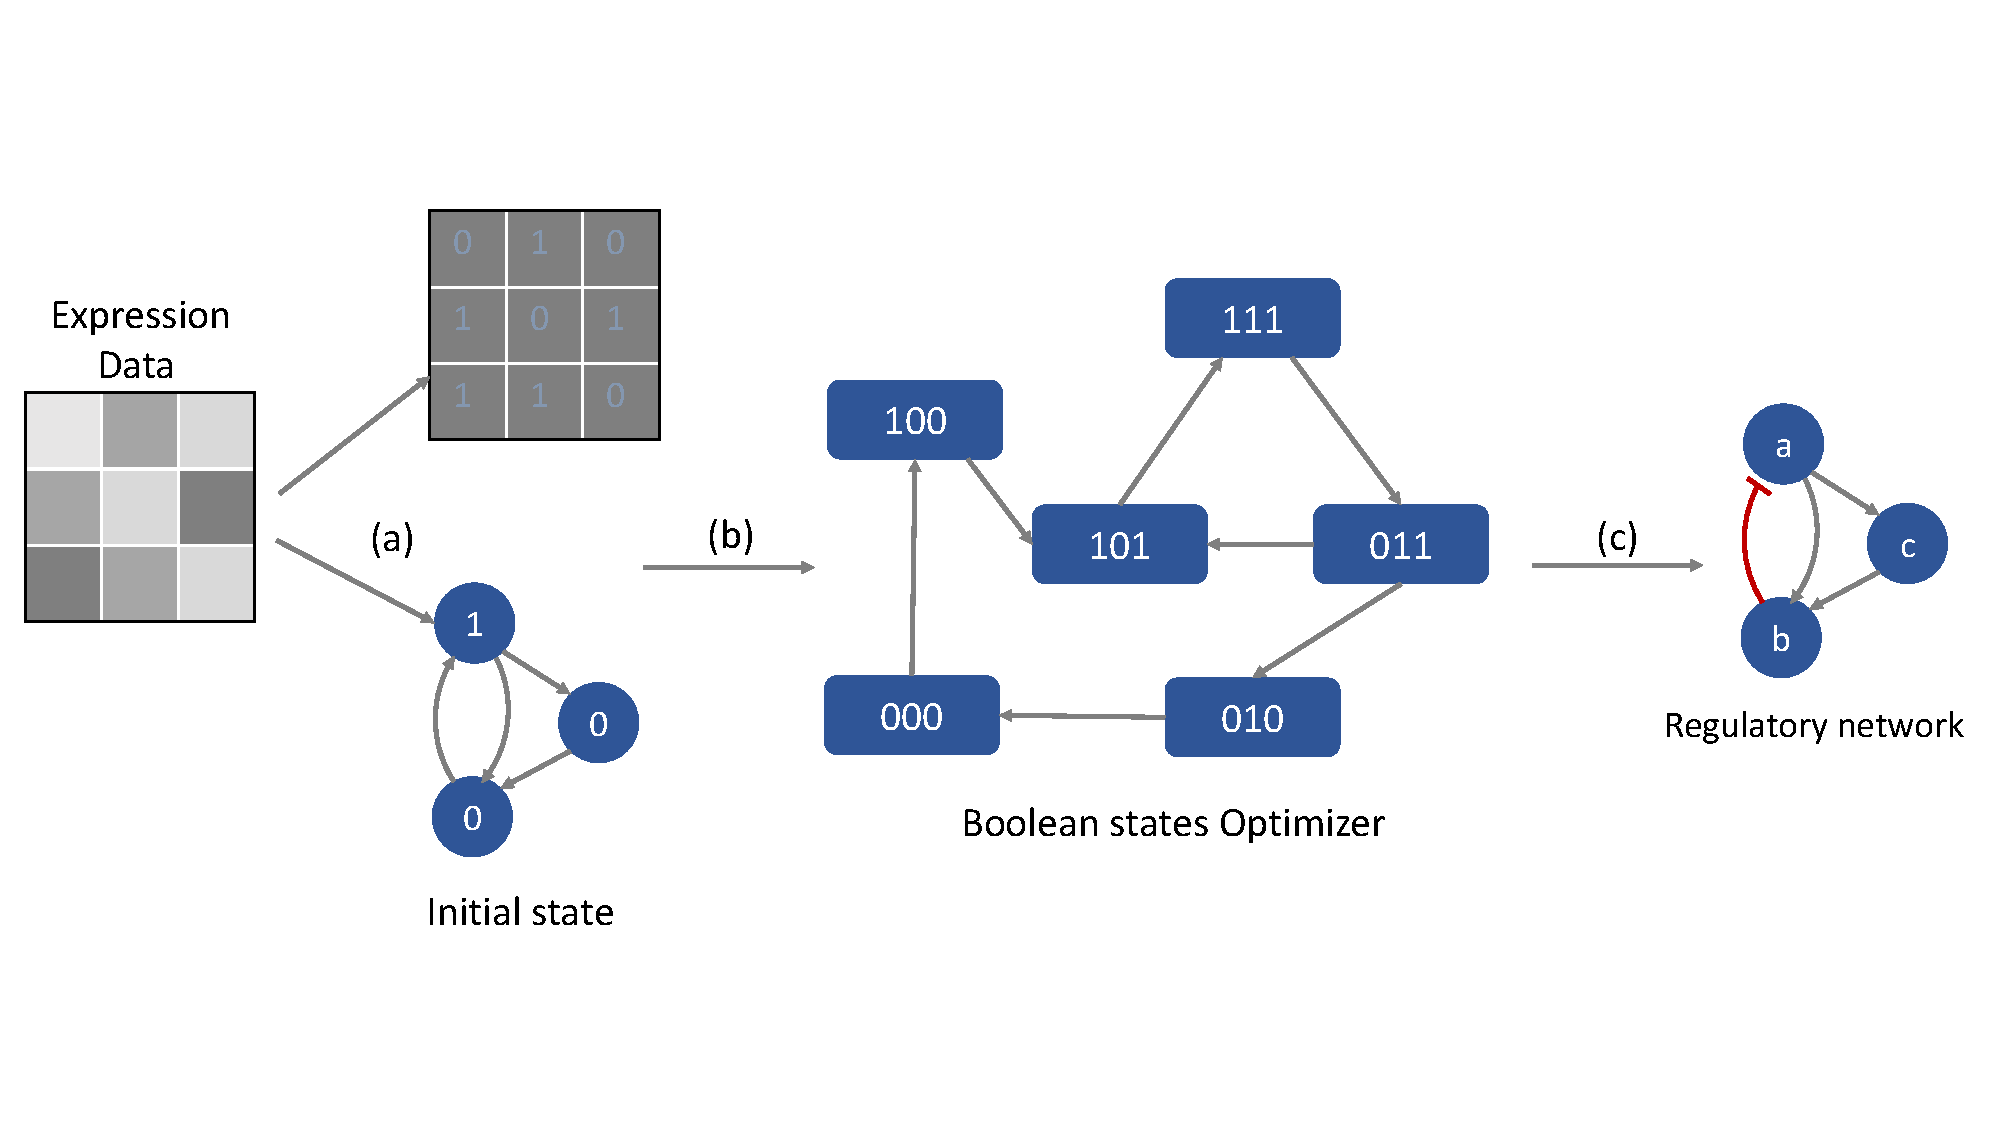
\includegraphics[width=0.9\textwidth]{introduction-bn.pdf}
    \caption{
        使用布尔模型的方法的整体工作流程。
        (a) 这些方法首先对基因表达数据进行二值化,然后生成初始布尔状态。
        (b) 这些方法针对二值对模型的状态进行优化。
        (c) 这些方法输出带有激活和抑制边缘的GRN或一组布尔函数。
    }
    \label{fig:pre-bn}
\end{figure}

基于布尔网络模型的主要工作包括:
 Kauffman \cite{kauffman2003random} 提出布尔网络的分析框架;
Akusu 等 \cite{akutsu1999identification} 证明了布尔网络推理所需要的最少样本数量;
Liang 等 \cite{liang1998reveal} 开发了 REVEAL 算法。
Shmulevich 等 \cite{marshall2007inference} 将马尔可夫链 (Markov Chains) 和布尔网络结合起来,引进了概率布尔网络模型 PBN (probabilistic boolean networks),
比标准布尔网络模型有了更多的优越性。
在单细胞 RNA-seq 测序数据上,
Chen 等 \cite{chen2014single} 开发了 SingleCellNet,
采用遗传算法从预期的轨迹通过细胞状态构造概率布尔模型, 他们采用的布尔规则直接来源于文献。
Moignard 等 \cite{moignard2015decoding} 提出了 SCNS 算法,通过状态转换图分析轨迹来推断一个异步布尔模型。
连接状态转换图在这个算法中起着至关重要的作用,但是它很难从单细胞表达数据中获取。

布尔网络模型是最简单的网络模型,它通过布尔变量和布尔逻辑实现。
布尔网络建模时, 把基因的表达水平离散化成单一的表达和不表达两个数值,
而在现实的生物系统中,基因的表达过程是连续的,
对基因数据进行离散化时不可避免的会丢失很多重要的表达信息,
布尔网络模型不能完全捕获复杂的系统行为 \cite{lee2009computational};
网络中一个节点更新,会使得所有节点同步更新,而在实际的基因表达过程中,更新是异步进行的。

(2) 微分方程模型

微分方程模型是一种连续的确定模型, 具有强大灵活的优点,
通过抽象基因间的时序调控变化,相比布尔网络来讲, 适合描述更加精细的调控关系,可以较好地建模基因表达数据 \cite{gardner2003inferring,di2005chemogenomic,bansal2006inference, honkela2010model,lu2011high,li2011large}。
另外,通过加入新的变量,微分方程模型可以进一步描述环境变化对于基因表达水平的影响。

Chen \cite{chen1999modeling} 最早使用微分方程系统作为基因表达调控网络模型。
若采用变量 $e_i$ 表示第 $i$ 个基因在 $t$ 时刻的表达水平, 则 $n$ 个基因之间的调控关系可以用微分方程描述如下:
\begin{equation}
\frac{{d_{e_i}}}{{dt}} = f_i (e),1 \le i \le n
\end{equation}

式中 $\frac{{d_{e_i }}}{{dt}}$ 代表基因调控网络建模中,
第 $i$ 个基因在 $t$ 时刻表达水平的变化率,向量 $e=[e_1,e_2,...,e_n]^T$ 则描述基因表达水平。
式中 $f_i(e)$ 的表现形式表明了基因之间的调控机制和作用方式,也就是调控网络的结构。
调控函数 $f_i(e)$ 最简单的形式是线性函数,可以表示为:
\begin{equation}
\frac{{d_{e_i }}}{{dt}} = \sum\nolimits_j {w_{ij} e_j} { + b_i } ,1 \le i \le n
\end{equation}

调控网络系统中各个基因之间的调控关系可采用参数 $w_{ij}$ 表示,
激活、抑制和无调控关系分别对其取值为正、负或为零, $b_i$ 表示基因的基础活性。
基因之间复杂的非线性作用关系可利用非线性的调控函数 $f_i(e)$ 进行刻画和说明。
比如 Sigmoid 函数 (S型函数),来引入必要的非线性,具体表达形式为:

\begin{equation}
\frac{{d_{e_i } }}{{dt}} = AS(\sum\nolimits_j {w_{ij} e_j } + b_i) - D_i e_i ,1 \le i \le n
\end{equation}

图 \ref{fig:pre-df} 展示了使用微分方程模型方法的整体的工作流程。
\begin{figure}[!htbp]
    \centering
    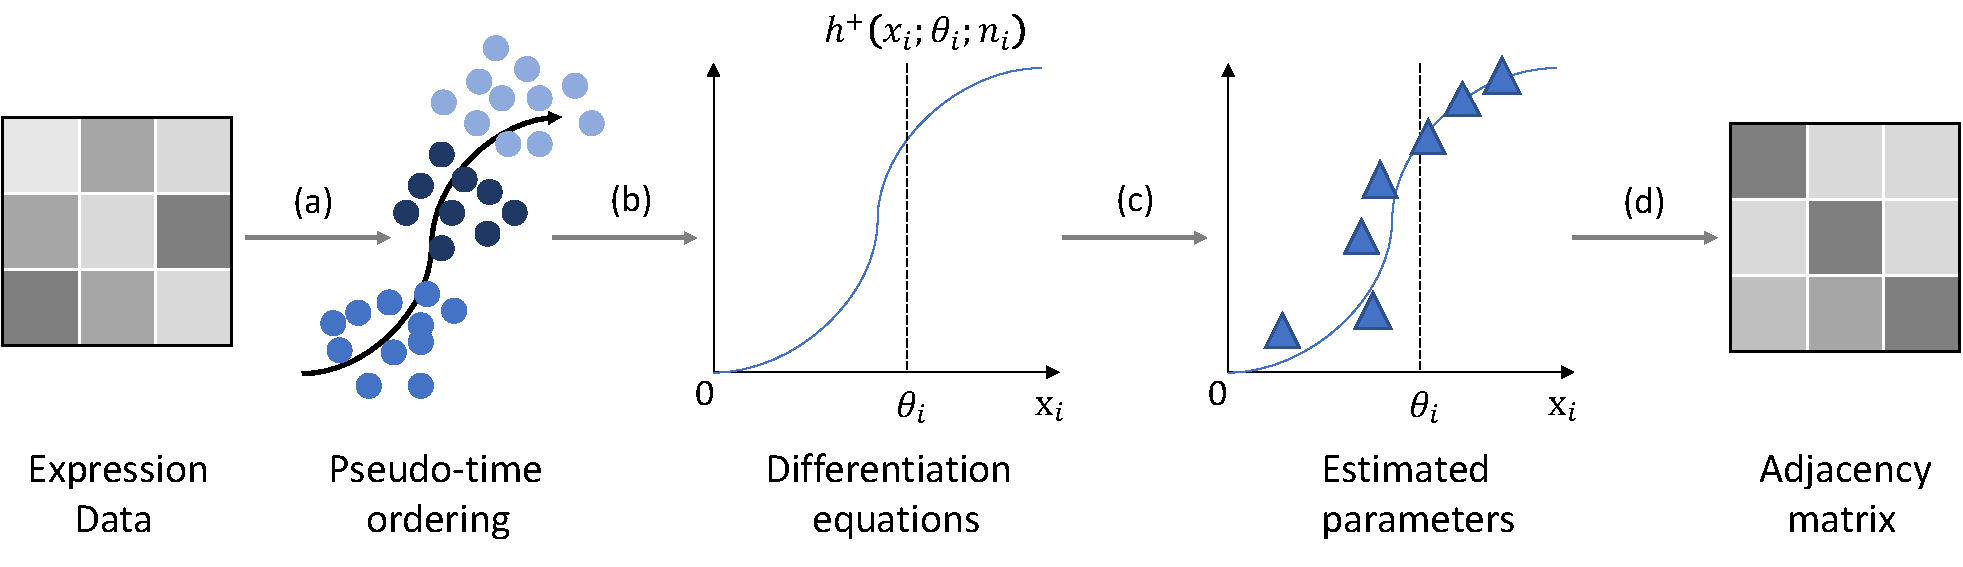
\includegraphics[width=0.9\textwidth]{introduction-df.pdf}
    \caption{
        基于微分方程的方法的整体工作流程。
        (a) 针对单细胞数据集利用外部算法或软件构建细胞间的伪时序, 或者直接采用数据集提供的时间标签特征。
         DNA 微阵列测序数据直接采用提供的时间标签特征。
        (b) 方法利用微分方程描述基因之间跟时间的关系。
        (c) 使用不同的优化技术进行参数估计。
        (d) 根据使用优化后的参数结合微分方程构建出基因之间的关系,输出关联矩阵。
    }
    \label{fig:pre-df}
\end{figure}

在单细胞测序数据集上, 
为了从时间序列数据构建网络, SCODE \cite{matsumoto2017scode} 和 SCOUP \cite{matsumoto2016scoup} 
分别引入 ODEs 和 SDEs 来计算基因之间的相关性。
SCODE 将某一基因在某一时间点的基因表达水平构建为对其他基因表达水平的线性依赖关系,
然后使用线性回归来估计基因之间的相关性矩阵;
SCOUP 则将各基因表达水平随时间的分化建模为一个连续的随机扩散 Ornstein-Uhlenbeck (OU) 过程,
其中的某一个基因在某一时间点的表达量可以通过当前 OU 过程的正态分布来估计,
然后利用计算出的所有细胞的 z 值得到基因之间的相关性。

微分方程其主要的优点在于强大灵活,有利于描述基因网络中的复杂关系,能够很好的表现出基因之间的连续动态关系;
其缺点是难以适应中大型网络的构建, 计算量较大, 捕捉基因表达数据中包含的随机信息欠佳。

(3) 贝叶斯网络

贝叶斯网络 (Bayesian Networks, BNs) 是一种重要的概率模型 \cite{kim2003inferring,zou2004new,chen2006effective,needham2007primer,lo2015high},
由条件概率分布和网络结构两部分组成。
自从 Friedman 等 \cite{friedman2000using} 将贝叶斯网络应用到基因调控网络的重构中后,
贝叶斯网络在生物学上的应用越来越广泛,成为现今构建细胞调控网络最有效的方法之一。
在贝叶斯网络模型中变量之间的结构用有向无环图 (directed acyclic graph, DAG) 来表示,
变量之间的关系使用联合概率分布来描述。
相对于布尔网络的粗放定性,微分方程的精细定量,贝叶斯网络模型可看做这两者的折衷。

Cooper 等提出的 K2 算法 \cite{cooper1992bayesian} 是一个基于搜索评分的经典算法,
该算法为评价模型与数据的符合程度,
首先在给定先验信息和节点顺序的情况下,通过后验概率作为评分标准并利用贪婪搜索方法找出最佳网络结构。
%Peer \cite{pe2001inferring}等人将贝叶斯网络技术用来处理调控网络中的扰动。
% 他们首先将数据离散化后根据评分函数挑选出最佳的的基因网络。
Imoto 等 \cite{kim2003inferring} 用非参数回归模型来解决离散化造成的阀值选取与信息丢失问题,
Imoto 等采用这一模型能获得基因之间的线性与非线性结构特征。
Jansen 等 \cite{jansen2003bayesian} 为利用贝叶斯网模型构建调控网络,
分析和计算各类基因表达数据以及蛋白质相互作用数据,并通过生物实验验证了模型的预测结果。
2004年 Friedman 等 \cite{friedman2004inferring} 为构建静态基因调控网络,
首次基于微阵列数据将贝叶斯网络模型用来预测基因调控关系。
Hartemink 等 \cite{hartemink2005reverse} 采用 BDe 评分测度作为学习的目标函数,
通过对基因表达数据进行离散化及模拟退火算法来构建基因调控网络。
Werhli 和 Husmeier \cite{werhli2007reconstructing} 将基因表达数据与来自多种数据源的先验生物学知识结合起来使用贝叶斯网络模型利用马尔科夫链蒙特卡洛 (MCMC) 抽样方案来抽样来自后验分布的超参数,
这种与多数据源的结合降低了基因调控网络参数学习的误差率,提高基因调控网络重建的准确性。
Yavari 等人 \cite{yavari2008gene} 根据基因本体将基因进行聚类,
并使用贝叶斯网络推断共聚簇基因之间的相互作用。
这种方法可以解决由于基因数目增加而导致的结构数量指数增加的问题。 
此外,他们还提出了一种在推理过程中使用共聚基因之间的互相关性的新方法。
共聚簇基因之间的互相关性为贝叶斯网络提供了时间延迟信息。 
由此模型产生的精度和灵敏度均有提高,而且结果表明这种模型适合对大规模基因进行建模。
杨等人 \cite{yang2011bayesian} 建议使用稀疏图搜索 (SGS) 算法减少贝叶斯网络的计算时间。
SGS算法利用迭代统计独立性测试和搜索技术来寻找最佳的网络结构。
最佳的基因调控网络是使用搜索-打分和基于约束两种方法混合产生的。
基于搜索和打分是使用优化技术在所有候选网络上搜索最佳网络结构并打分用来评估网络质。
基于约束的方法通过应用条件独立性检测来取代传统的统计或信息论度量来检测边的存在。
结果表明,他们提出的方法提高了准确性和计算效率。
Tan 和 Mohamad \cite{kunga2012using} 使用贝叶斯网络结合爬山法和 Efron 的 bootstrap 抽样方法来构建基因调控网络。
他们首先使用最小局部平方 (LLS) 插值算法来处理微阵列数据集中存在的缺失值, 
然后采用贝叶斯网络建立网络模型并采用爬山算法进行学习, 
bootstrap 抽样方法被用来抽取高置信度的边集合。
他们的基因调控网络构建方法获得了较高的真阳性率, 并且揭示了基因之间更新的关系。 
Young 等 \cite{young2014fast} 提出一种基于贝叶斯网络的 ScanBMA 算法,
该方法采取数据变换和新的策略在模型空间搜索时高效快速,
可应用于大规模的基因调控网络构建。

贝叶斯网络模型的优点是灵活性好, 具有从数据中推导模型的能力, 能够自然地融入先验知识并能用专家知识和数据挖掘来改进模型的性能;
可以通过借助问题领域自身结构特征和变量间直接影响的局部性, 同时使用条件独立的数学概念, 将聚合概率分布的计算问题,分解为若干局部条件概率分布的计算问题;
模型结构和参数具有明确的含义可解释性好, 具有良好的学习能力; 能很好地处理隐变量和数据缺失问题。
研究发现与关联网络相比, 贝叶斯网络在识别准确度上常有更优异的表现, 尤其是在网络规模较小时。
其不足之处是: 许多贝叶斯网和动态贝叶斯网常采用离散模型, 对基因表达数据离散化导致损失了部分信息,
同时也降低了网络构建的准确度;
没有时序的概念,特别是对于存在伪时序的单细胞数据集而言,不能明显地表现基因调控网络的动力学特征。

(4) 动态贝叶斯网络

动态贝叶斯网络 (Dynamic Bayesian Network, DBN) 模型是在静态 BN 网络模型中引入时间因素而形成的动态网络 \cite{dondelinger2010heterogeneous,grzegorczyk2010improvements}。
DBN 可以很好的表示随机系统的动态特性,也使用图模型的方式来表示模型中随机变量之间的概率依赖关系 \cite{hecker2009gene}。
DBN 更好地刻画了基因调控网络的动态特性,善于处理非线性关系和由随机现象引起的不确定性,能够描述基因之间的负反馈调控过程,
相比于静态贝叶斯网它能够克服其有向无环的缺点,具有很好的概率推理能力和知识表达能力,使得模型的预测精度进一步提高。

Friedman 和 Murphy 等 \cite{friedman2004inferring} 考虑到了基因调控存在一定的时延性,
从理论的角度分析了 DBN 从时序基因表达数据构建基因调控网络的问题, 提出用动态贝叶斯网络模型分析时序基因表达数据。
Smith 等 \cite{smith2006computational} 用动态贝叶斯网络模型来分析微阵列数据,
结合了基因调控的负反馈与时延因素, 因此需要采用网络中不同节点来表示同一基因不同时间点的表达向量。
Wu和Liu等 \cite{wu2008dynamic} 改进了动态贝叶斯网络构建方法,使用了 MCMC 和带重启的贪心爬山算法两种不同的模型搜索方法。 
两种方法在时间效率上不相上下,与带重启的贪心爬山算法相比 MCMC 具有更高的预测精度。
Song \cite{song2009keller}结合微阵列数据与基因关系的先验知识在 DBN 上提出新的数据整合模型,利用并行算法,构建基因调控网络。
Kim 等 \cite{del2010efficient} 也在这方面做了大量的工作,
并结合线性或非线性模型以及相应的生物学知识对动态贝叶斯网络进行了改进。
Norbert \cite{netrapalli2010greedy} 为从基因扰动型实验数据中学习动态贝叶斯网络,
利用 Husmeier \cite{werhli2006comparative} 提出的离散化方法来对基因表达数据进行预处理,
并使用 BDe 测度来进行评分搜索,最终构建动态贝叶斯网络, 这种搜索方法实现了减少学习时间,降低计算的时间复杂度的目的 \cite{hurley2011gene}。
Grzegorczyk 和 Husmeier \cite{grzegorczyk2010improvements} 通过将多变点过程与可逆跳跃马尔可夫链蒙特卡罗方法 (RJMCMC) 结合,改进了基于动态贝叶斯网络构建的方法。 他们通过引入动态编程方案来优化RJMCMC上的收敛性,该方法从正确的条件分布对变化点进行采样。 
此外,引入了贝叶斯聚类的新方法以促进节点之间的信息共享, 使得模型复杂度能够自动调整。
Chai 等 \cite{chai2012inferring} 提出了缺失值插补的动态贝叶斯网络模型,
利用缺失值插补来提高基因调控网络构建中的计算效率,
同时通过限制潜在调控因子的表达变化来缩短计算时间。
Vinh 等 \cite{vinh2012gene} 将动态贝叶斯网络方法与基于时间序列表达数据的基因调控网络构建的全局最优化相结合,
他们在全局优化框架上使用互信息测试来学习高阶带延时的基因相互作用。
他们的方法能够改善动态贝叶斯网络只适合于小规模网络的缺陷,
同时能够避免动态贝叶斯网络结构学习容易陷入局部最优的状况。

(5) 关联网络

关联网络 (relevance network) 主要借助基因表达数据间相关性的计算来构建网络模型。
相关性分析是构建基因调控网络最常见的方法之一。
计算基因间的相关性常通过互信息、皮尔逊相关系数等测度来进行。
主要思路是: 对于预先设定的阈值,若基因间相关性不在阈值范围内,则在网络中基因间有边相连。
若两基因间具有相同或相近的调控机制,则两个基因相关性较高,
尤其是,对于同一转录因子的靶基因或同一条生物通路上的基因,它们的相似度或相关性较高。

皮尔逊相关系数 (PCC) 是一种线性相关系数, 它反应了两个变量间的线性相关程度。
设 $X$,$Y$ 为随机变量, $pcc(X,Y)$ 定义如下:

\begin{equation}
pcc(X,Y) = \frac{{\sum\limits_i {(x_i -\bar x_i )(y_i -\bar y_i )} }}{{\sqrt {\sum\limits_i {(x_i  - \bar x_i )^2 } } \sqrt {\sum\limits_i {(y_i  - \bar y_i )^2 } } }}
\end{equation}

其中, $\bar x_i$、$\bar y_i$ 分别是 X、Y 的均值。
 $pcc(X,Y)$ 的取值在 -1到 1之间。
当 $pcc(X,Y)$ 为 -1 或者 1 时, 表示两个变量完全相关;
当 $pcc(X,Y)$ 为 0 时, 表示两个变量完全无关。

PCC 被广泛用于评估变量之间的线性关系 \cite{stuart2003gene},但在不借助其他信息的情况下无法区分直接关系和间接关系,而偏相关分析法 (PC) \cite{baba2004partial} 通过考虑附加信息条件来有效区分直接和间接关系。
另外, Barabási 等 \cite{barzel2013network} 提出了一个基于动态关联性的方法,该方法通过消除网络中的间接影响进行直接关联性和间接关联性区分; 
Feizi等 \cite{feizi2013network} 提出了利用网络卷积去除所有关联之间的综合效应区分直接和间接关联性。
这两种方法只能测量线性直接关联性,
但无法测量非线性关联性, 而非线性关联性在许多非线性系统比如生物系统中发挥着重要的作用。
基于 PCC 和 PC, 距离相关性 \cite{szekely2007measuring,kosorok2009brownian} 和部分距离相关性 (Pdcor) \cite{szekely2014partial} 被提出用于度量随机向量间的相关性,这些统计量对于依赖偏离很敏感。
Pdcor 的评估存在假阳性,即当向量 $X$ 非条件独立时, Pdcor(X;Y|Z) 也有可能为零 \cite{szekely2014partial}。

互信息 (Mutual Information, MI) 常用来刻画和描述两个系统间的统计相关性,或通
过熵来反应一个系统中蕴含的另一个系统信息量的大小, 设 $P(x)$ 是 $X=x$ 的概率,
则随机变量 $X$ 的熵定义为 \cite{cover2012elements}:
\begin{equation}
    H(X) = - \sum\limits_x {P(x)\log _2 P(x)} 
\end{equation}

设 $P(x,y)$ 是 $X=x$, $Y=y$ 时的联合概率,则 $X$, $Y$ 的联合熵定义为:
\begin{equation}
    H(X,Y) =  - \sum\limits_x {\sum\limits_y {P(x,y)\log _2 P(x,y)} } 
\end{equation}

随机变量 $X$ 和 $Y$ 的互信息为:
\begin{equation}
    MI(X,Y) = H(X) + H(Y) - H(X,Y) = \sum\limits_{i,j} {P(x_i ,y_i )\log \frac{{p(x_i,y_i )}}{{p(x_i )p(y_i )}}} 
\end{equation}

需要注意的是在基因调控网络构建中由于基因表达数据是连续的,而互信息在计算时需要离散化,
一般使用 B-样条平滑和离散化方法来进行计算 \cite{daub2004estimating}。
由于互信息能够捕获有效捕获变量间的非线性相关性,
因此在复杂的基因调控网络相互作用构建中其应用十分广泛 \cite{brunel2010miss,zhang2011inferring}。

图 \ref{fig:pre-gc} 展示了关联网络模型方法的整体的工作流程。
\begin{figure}[!htbp]
    \centering
    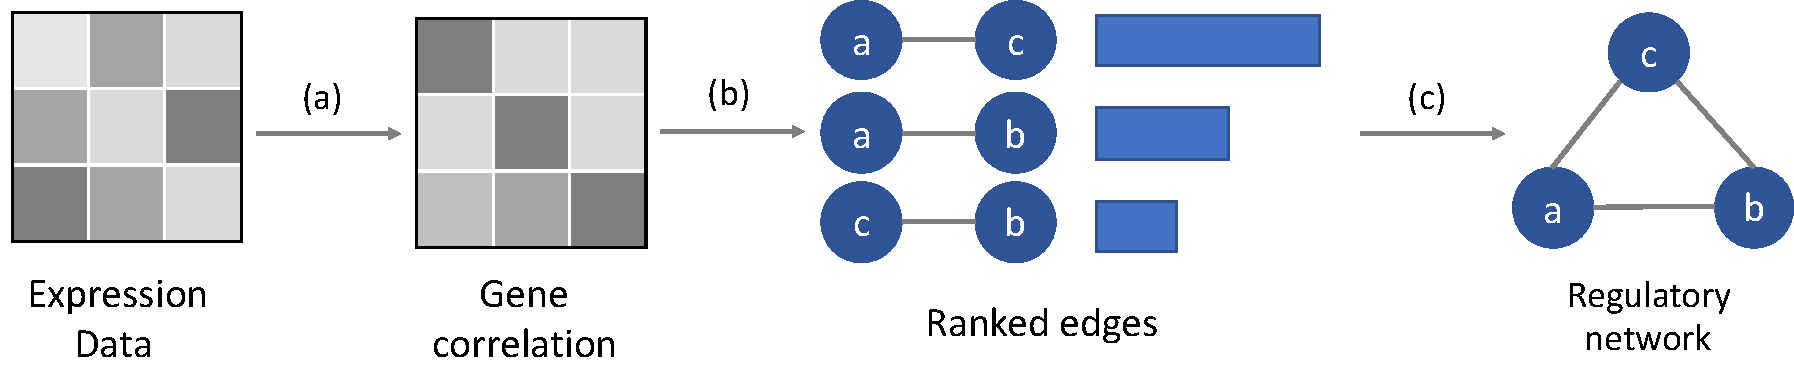
\includegraphics[width=0.9\textwidth]{introduction-gc.pdf}
    \caption{
        利用基因表达相关的方法的整体工作流程。
        (a) 首先通过计算每个基因对的表达相关性来初始化边缘的权重。
        (b) 进行假设检验,估计每个边缘的显著性,然后使用预定义的显著性阈值去除被认为不显著的边缘。
        (c) 方法输出最大的连接分量。
    }
    \label{fig:pre-gc}
\end{figure}


Butte 等 \cite{basso2005reverse} 首先利用互信息计算所有基因对之间的相关性,然后设置互信息阈值。
为构建关联基因调控网络, 通常定义高于阈值的基因对之间存在关联并使用边连接起来构成网络。
Margolin 等 \cite{margolin2006aracne} 提出的 ARCANE 采用 Data Processing Inequality (DPI) 来过滤间接作用边。
Faith 等 \cite{faith2007large} 提出的 CLR 方法使用互信息的经验分布来过滤间接作用边。
Meyer 等 \cite{meyer2007information} 提出的 MRNET 方法使用最小化冗余特征选择算法 \cite{peng2005feature},
在计算后的互信息网络上对每一个目标基因选择一个同目标基因关联最强但与已经候选的基因集合冗余性最低的基因,这个过程不断进行迭代。
Altay 等 \cite{altay2010inferring} 提出的 C3NET 和其扩展算法 BC3NET \cite{de2012bagging} 结合一个最大化的步骤来估计互信息从而使预测更准确。

MI 被广泛用于评估变量之间的非线性相关性,
它是基于统计独立性进行计算。
需要注意的是,在只有联合概率时无法计算直接变量之间的 MI,
并且 MI 和 PCC 一样有假阳性 \cite{frenzel2007partial,schreiber2000measuring}。
Zhao 等提出了条件互信息 (Conditional Mutual Information, CMI) \cite{zhang2011inferring} 和部分互信息 (Part Mutual Information, PMI) \cite{zhao2016part},
这两个测度在互信息上引入了条件计算的机制减少了假阳性边,
能有效检测变量之间非线性的间接或直接的相互作用。
他们将这两个测度与基于贪心策略的路径一致性算法 (Path Consistency Algorithm, PCA) 结合起来先后提出了 PCA-CMI \cite{zhang2011inferring} 和 PCA-PMI \cite{zhao2016part}。

在单细胞测序数据集上,
Yu 等提出了 NLNET 方法\cite{yu2013hierarchical}, 
两个基因之间的相关性被定义为基于条件有序列表 (Conditional ordered list, DCOL) 的距离,
其中基因 G1 到基因 G2 的距离取决于通过 G1 中所有样本的表达顺序。
NLNET 使用的这种距离度量没有考虑到的点是,真实生物网络中的一个基因可能与多个基因相互作用。
Thalia 等 \cite{chan2017gene} 提出了高效的 PIDC 算法,
该算法利用偏信息分解 (partial information decomposition, PID) 测度来衡量基因之间的关系。
Guo 等 \cite{guo2015sincera} 提出了 SINCERA 方法, 该方法利用低阶偏相关性 (low-order partial correlation),可以在测量中涉及两个以上的基因,是一种更符合实际的方式来呈现复杂网络的相互作用。
在 SINCERA 方法中,给定第三个基因 G3,基因 G1 和基因 G2 之间的相关性是 G1 与 G3 的线性回归
所产生的残差与 G2 与 G3 的线性回归所产生的残差之间的相关性。
SINCERA 假设基因之间存在线性依赖关系,并使用最小平方估计来计算目标基因和条件基因的回归系数。

可以看出,虽然关联网络建模操作简单易行,但不管是基于 PCC、MI 还是 PID 等测度构建的网络极其容易引进假阳性边。
虽然各种方法都站在不同的角度来尽量减少假阳性边来提高网络构建的准确性,
但是随着网络规模的扩大这种状况还是在不断恶化,网络构建的准确性急剧下降。

(6) 回归方法

近年来在 DREAM 系列竞赛的推动下,利用机器学习回归模型进行基因调控网络的构建方法大量地涌现出来。
这类方法本质上可以看作是关联网络模型的延伸,
但是与关联网络只关注量化相互作用不同的是,回归方法能够构建出基因之间的相互作用方向。
回归模型将基因调控关系转化为机器学习特征选择的问题,
即是将靶标基因的表达看作是调控基因表达之间的相互线性作用或者非线性作用的结果,
然后采用 bagging 或者 boosting 的做法,构建出最终的基因调控网络。
它们应用在基因调控网络构建上优点是计算效率高,网络构建准确率高;
缺点是一些非线性的模型可解释性较低参数意义不明确,并且缺少对生物结构的支持。
回归模型成功应用于基因调控网络构建中的典型算法包括基于随机森林的 GENIE3 \cite{Huynh-Thu2010},
基于 Lasso 回归的 TIGRESS \cite{Haury2012}。
在处理时间序列数据上有 GENIE3 的扩展方法 GENIE3-lag \cite{huynh2012machine},
与扩散模型相结合利用随机森林来学习隐含参数的 Jump3 \cite{Huynh-Thu2014}。

在单细胞 RNA-seq 测序数据集上, 
SCENIC \cite{aibar2017scenic} 融合了 GENIE3、 RcisTarget 和 AUCell 三个算法来在单细胞测序数据上实现了基因调控网络的构建和基因的聚类。
单细胞 RNA-seq 也能产生基于时间序列的 RNA-seq 数据。
与传统的时间序列数据相比,基于单细胞的时序数据在单个时间片上产生了更多的样本,测序的总体成本也变得十分昂贵。
因此也有很多方法利用原始数据构建出伪时序 (pseudo-time ordering) 后,再利用回归方法构建基因调控网络。
LEAP \cite{specht2017leap} 简单地使用皮尔逊相关性来计算每个时间窗口的基因之间的相关性。 
然后,它通过收集所有时间窗口内所有基因对的最大相关性来合并所有相关矩阵。
SINCERITIES \cite{papili2017sincerities} 利用基因在不同时间片上的表达分布之间的距离来构建基因的表达矢量,
然后使用格兰杰因果关系 (Granger causality) 的思想结合线性回归模型来构建基因调控网络。
SINCERITIES 并没有直接来计算在每个时间窗口中基因间的相关性。
SCIMITAR \cite{cordero2017tracing} 使用连续的多变量高斯混合模型对数据进行建模,
然后使用期望值最大化 (EM) 算法估计参数。
EM 算法估计了每个分布的参数,以及一个细胞属于每个分布的可能性。
SCIMITAR 从混合模型的协方差矩阵中计算出每个伪时间的相关矩阵,
然后该方法通过计算协方差矩阵之间的距离来计算相似度矩阵,
最后使用相似度矩阵的频谱聚类 (Spectral Clustering) 来确定整个时间轨迹的发展阶段。
对于每个发展阶段,该方法通过对该阶段的相关矩阵进行平均,最终输出共识网络。
SINGE \cite{deshpande2019network} 使用回归模型来确定一个时间窗口内两个基因之间的相关性。
对于每个目标基因,该方法利用基于核函数的格兰杰因果关系 (Granger causality) 回归来计算该基因与所有其它基因的相关性。
然后采用 Borda 计数聚合方法 \cite{van2000variants} 来对调控边打分,
该方法偏重于多次格兰杰检验一致性排名靠前的边,对两个基因之间的连接进行随时间的排序。
上述四种方法中, SCIMITAR 自身能直接从输入的数据中构建出细胞的伪时序, 
而 LEAP、SINCERITIES 和 SINGE 都依赖用户在输入时提供细胞的时间排序。

\subsection{主要研究工作}
本课题的主要研究内容是基因调控网络构建。
从系统生物学的角度出发,通过计算方法研究基于 DNA 微阵列数据以及单细胞 RNA-seq 测序数据上的基因调控网络的构建、评估及其在复杂细胞类型分析等生物问题中的应用。
本文以复杂网络理论、信息论和机器学习方法为基础,以数据的结构特性和数据本身的特点为研究对象,
构建合适的网络构建模型和调控网络构建方法,
并同已有的方法进行评估和对比。

(1) 基于互信息的网络构建算法研究

通过对基于信息理论互信息的网络构建算法进行研究后发现,
由于原始数据中存在的外部噪声、
网络结构中的拓扑稀疏性和非线性基因之间的依赖等因素,
现如今这类方法在网络构建中会引入冗余的依赖关系。
特别是随着网络规模的增加,这些方法的表现大幅降低。
本文提出了一种新的基于互信息的网络结构构建方法 Loc-PCA-CMI:
首先识别局部重叠基因簇 (local overlapped gene clusters),
然后基于条件互信息 (PCA-CMI) 的路径一致性算法构建每个簇的局部网络结构,
最终通过聚合局部网络结构,也就是基因之间的依赖性网络,来构造最终的 GRN。

(2) 基于数据驱动的网络构建算法研究

最近关于数据驱动的动态网络构建的研究为我们构建 GRN 提供了新的视角。
当前基于数据驱动的动态网络方法无法构建全局网络,
本文提出了一种改进 ARNI 和抽样的基因调控网络构建方法 D3GRN。
% 该方法使用了抽样的策略 (bootstrapping),
% 将每个目标基因的调控关系转化为函数分解问题并利用揭示网络相互作用的算法解决各个子问题。
% 为了弥补数据驱动方法无法构建全局网络的缺陷,
% 我们最后采用了抽样策略和基于面积的评分方法来构建最终的网络。
该方法将针对每个目标基因的调控网络构建转化函数分解问题,
采用改进的数据驱动的方法 ARNI 来推断各个子网络。
该方法结合了抽样策略和基于面积的评分方法来聚合这些子网络从而构建最终的全局网络,
克服了传统的数据驱动方法无法构建全局网络的缺陷。

(3) 基于矩阵分解的单细胞基因调控网络方法研究

识别细胞类型特征和细胞的基因表达活动程序 (如生命周期过程、对环境因素的反应) 对于理解细胞和组织的组成至关重要。
虽然单细胞 RNA-seq 数据可以量化成单个细胞中的转录本,
每个细胞的表达谱可能是这两种类型的程序的混合物,使它们难以分离。
在这里, 本文提出了一个使用矩阵分解的算法 WSSMFA 来解决这个问题。
通过模拟表明, 我们提出的 scGRNHunter 方法可以准确地构建出身份和活动性的子程序, 
并在此基础上构建基因调控网络。


(4) 面向单细胞 RNA-seq 数据的单细胞细胞类型识别方法研究

单细胞数据聚类是单细胞数据上游分析的核心任务, 
在很大程度上是构建与细胞类型相关的基因调控网络的必要步骤。
相似性学习是当前单细胞聚类算法研究的重点。
针对当前单细胞 RNA-seq 数据集上细胞聚类不够准确鲁棒的问题,
本文提出了一个基于随机森林相似性学习的聚类方法 RafClust。
该方法使用多种相关性度量方法来刻画细胞的特征, 
然后使用随机森林回归模型进一步学习细胞与细胞之间的相似性矩阵,
最后采用层次聚类来决定细胞的最终类别。

针对超大规模 scRNA-seq 数据集,
现有的寻找稀有细胞的算法大部分依赖单细胞聚类方法,非常耗时或耗费内存。
在上一个细胞聚类工作的基础上,本文提出了一种高效准确的基于孤立森林的稀有细胞识别方法 DoRC。
DoRC 产生的稀有度分数可以帮助生物学家们只关注超大规模 scRNA-seq 数据内一部分的细胞, 也就是稀有细胞,
然后结合细胞聚类方法 RafClust 进一步区分稀有细胞类型和进行后续分析。

这四个方面的研究工作涉及到五种方法,它们之间的在研究思路上的宏观关系如图 \ref{fig:pre-structure} 所示。
这五种方法涉及到两种类型的基因测序技术数据, 无向网络构建的有 Loc-PCA-CMI 方法, 有向网络构建有 D3GRN 和 scGRNHunter 两种方法。 
% 由于 scGRNHunter 涉及到与单细胞聚类相关的讨论, 我们首先提出了单细胞聚类方法 RafClust。
单细胞稀有细胞的识别方法 DoRC 中利用了 RafClust 来确定稀有细胞的细胞类型,
一定程度上可以认为单细胞稀有识别方法 DoRC 是 RafClust 方法的一个具体的应用场景。
\begin{figure}[!htbp]
    \centering
    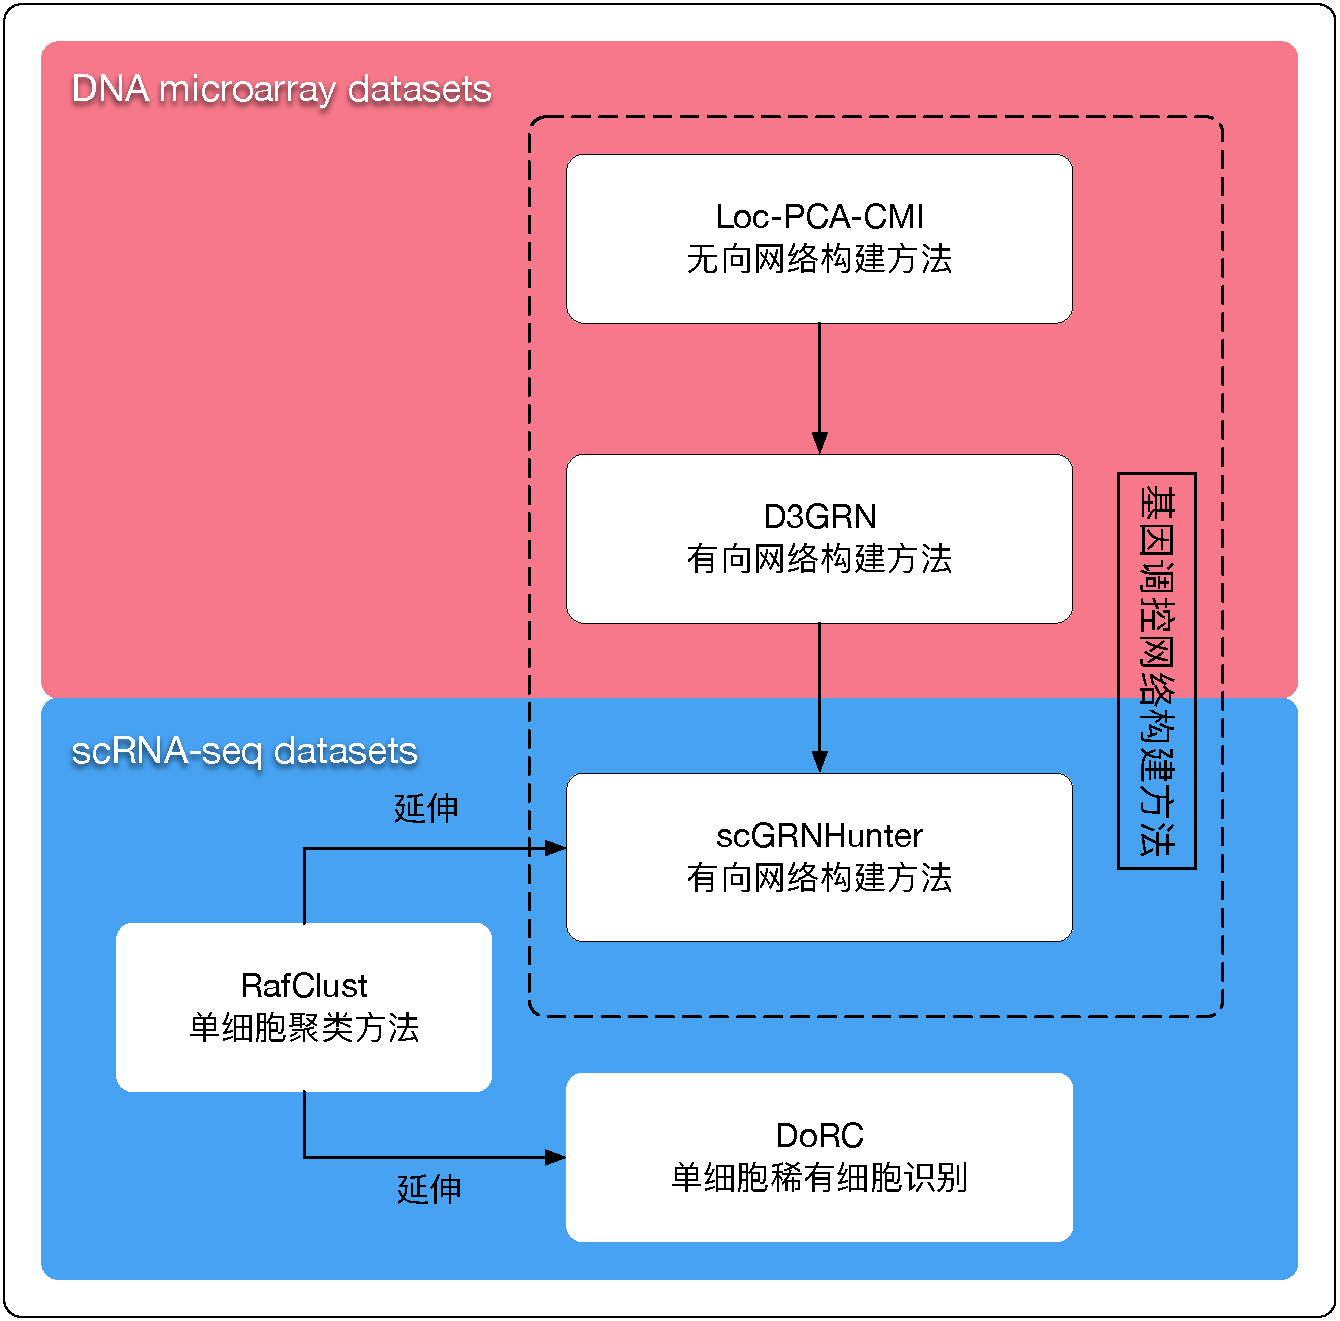
\includegraphics[width=0.8\textwidth]{pre-structure-plus.pdf}
    \caption{本文主要研究工作的关系图。}
    \label{fig:pre-structure}
\end{figure}

\subsection{论文组织结构}

全文内容共六章,各章内容简述如下:

第一章 绪论。
主要描述了基因调控网络研究在目前的研究背景与意义, 国内外研究现状和发展动态。
最后,介绍本论文的研究工作,并给出全文的结构安排。

第二章 基于互信息和局部结构融合的基因调控网络结构构建方法。
主要介绍了基于互信息网络构建算法相关工作, 为了降低假阳性调控边的引入设计了 Loc-PCA-CMI 算法,详细介绍了算法细节,并对使用的数据集进行了介绍,之后对实验结果进行了讨论和总结。

第三章 基于数据驱动和抽样的基因调控网络构建方法。
主要回顾了当前最热门的基于回归的基因调控网络构建方法和数据驱动的动态网络构建方法的研究现状,
对比了 D3GRN 与其它几种方法的设计思路,并详细介绍了 D3GRN 的算法过程,
并对使用的数据集进行了介绍, 
之后对实验结果进行了讨论和总结。

第四章 基于矩阵分解的单细胞基因调控网络构建方法。
主要提出了一种新的单细胞数据上进行身份 GEP (gene expression program) 和活动 
GEP 进行构建的思路, 并以此为基础详细介绍了 scGRNHunter 的几个步骤, 其中重点介绍了矩阵分解算法 WSSMFA。
最后我们介绍了数据集, 并对实验结果进行了讨论和总结。

% 第四章 基于随机森林相似性学习的单细胞聚类方法。
% 主要回顾了当前单细胞 RNA-seq 数据集上的细胞聚类方法及其优缺点, 
% RafClust 的设计思路以及 RafClust 方法详细的流程,并对使用的数据集进行了介绍, 并对实验结果进行了讨论和总结。

% 第五章 基于孤立森林的单细胞稀有细胞识别方法。
% 主要回顾了当前稀有细胞识别方向的方法及其优缺点, 
% DoRC 的设计思路以及 DoRC 方法详细的流程, 并对使用的数据集进行了介绍, 并对实验结果进行了讨论和总结。

第五章 单细胞 RNA-seq 测序数据下的细胞类型识别方法。
这一章介绍了两种方法,一种是基于随机森林相似性学习的单细胞聚类方法 RafClust,
另一种是基于孤立森林的单细胞稀有细胞识别方法 DoRC。
主要回顾了当前单细胞 RNA-seq 数据集上的细胞聚类方法研究现状,详细介绍了 RafClust 的步骤,
并对使用的数据集进行了介绍,之后对实验结果进行了讨论和总结;
类似地,我们也回顾了稀有细胞的识别方法,详细介绍了 DoRC 的步骤,
并对使用的数据集进行了介绍,最后对实验结果进行了讨论和总结。

第六章 总结与展望。总结全文并对未来的研究方向进行了展望。